Creative AI, such as using deep learning models to generate paintings and music, has been a popular research domain.
Since creative activities are hallmarks of human intelligence, numerous works have attempted to replicate the creative process on machines.
For example, Pharmako-AI \citep{allado-mcdowell_okojie_2020} is a book co-written by K Allado-McDowell and GPT-3 \citep{gpt3} through exchanges between the human and the language model. 
Works like DALL-E, GLIDE, and DALL-E 2 tackle the problem of synthesizing images from short language descriptions, and these generative models have produced many imaginative and inspiring art pieces \citep{dallePaper,glidePaper,dalle2Paper}.
These work are often motivated by the vision to create machines that can interact with people and augment human creativity.  
Our work is driven by a similar vision: how can we build systems that can be creative like humans so that AI agents and people can participate in creative activities together and inspire each other. 

\begin{figure*}[!htb]
\centering
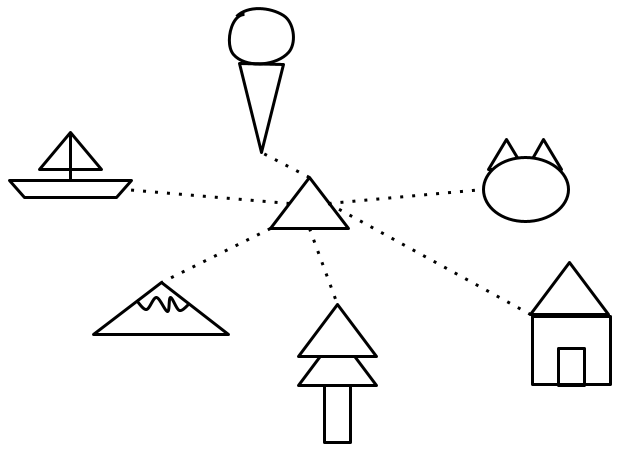
\includegraphics[width=.3\linewidth]{introduction/sketch_composition.png}  
\caption{Triangle is adapted and composed with other shapes to create sketches of different objects. The objects are, from top and in clockwise order: \textit{ice-cream, cat, house, pine tree, mountain}, and \textit{boat}.}
\label{introduction.composition}
\end{figure*}

Instead of generating realistic art works from a wide variety of language like DALL-E, we approach creativity from a different angle and investigate composing basic visual concepts in object sketches.
An example is illustrated in Figure \ref{introduction.composition}: a triangle can be the sail of a boat, the cone of an ice-cream, the left/right ear of a cat, the roof of a house, the canopy of a tree, or the body of a mountain. The same triangle is adapted to become different parts in sketches of different objects. 
While sketches contain much fewer details compared to their natural images counterparts, people are not any less creative when sketching. One could say that the abstractness allows for more creativity. 

Similarly, language descriptors can be composed to form new concepts applicable to different objects. For example, combining \textit{large} and \textit{round} or \textit{narrow} and \textit{oval} to describe different kinds of cat faces.
Many other objects can be \textit{large round} or \textit{narrow oval}: angel halo, glasses, mirror, plate, necklace charm, table, etc.
Moreover, there are multiple ways to describe the same sketch, depending on the person's viewpoint. \textit{What visual features does this cat sketch have?} Some people might pick up on its usual size; others might notice its slightly edged chin, and there are still others that focus on the long whiskers curving upwards. People are likely to provide a variety of responses.  
% Word meanings shift depending on the context they are applied in. For example, the word \textit{large} in \textit{a large scoop of ice-cream} and \textit{a large cat face} implies size at different scales and conjure up different imagery. The \textit{large} scoop of ice-cream is probably oveflowing from the little cone underneath with the melting ice-cream dripping from the side, while the \textit{large} cat face implies a chubby round face compared to the cute pointy ears at the top.          

We want to build systems that can compose basic shapes in a creative manner and understand how words are combined and adapted to describe different objects.  
In this thesis, we are interested in semantic parts in sketches and how people describe them. For example, a face sketch may contain four semantic parts: eyes, nose, mouth, and face contour, that can be drawn using various geometric shapes with different features. After examining existing sketch datasets, we found that they do not contain either language annotations or semantic part annotations. We explain the details of related sketch datasets in Chapter \ref{relatedWorkChapter}. To fill the gap and study this reuse of abstract concepts, we construct a dataset of language annotated face and angel sketches. We elaborate on the data collection process in Chapter \ref{dataChapter}.  

Moreover, we hope to understand the limits of current vision-language models, such as CLIP, or Contrastive Language-Image Pre-Training, which is trained on millions of image-text pairs. CLIP has been used extensively to provide a loss function for optimizing text-to-image synthesis models \citep{clipDrawPaper,dalle2Paper,styleganNadaPaper,styleCLIPPaper}. Despite the abundance of knowledge captured by CLIP's embedding space, we observed that CLIP, trained to associate natural images with their captions, has difficulty matching sketches from unseen categories with their part descriptions, suggesting that they might not understand that sketches from different categories are composed of parts different in semantics but share similar shapes and descriptions. We explain the details of CLIP and the fine-tuning process in Chapter \ref{modelingChapter}, and we analyze CLIP's performance and changes in its text embeddings after fine-tuning on our dataset in Chapter \ref{analysisChapter}. 
% For example, if we only train on face sketches and want to generalize performance to angel sketches that contain a new part, halo, CLIP does not recognize that \textit{circular face} and \textit{circular halos} are both circuls      

% % [B] 
% The ability to still get the idea across with such simple toolkit proves human creativity. We don't need complicated detailed realistic sketches, a few simple strokes are able to convey what we want to say. This type of creativity is innate. It is a creativity that we are born with: we start doodling as kids. We start scribbling on walls before knowing that we are re-creating our experience onto a canvas. It is the sort of creativity that lies on every one of us, and there is no high bar or artistic requirement to express this kind of creativity.

% % [B]
% Language creates space for imagination. Language creates room for creativity. The ambiguity in language. Large face. How large. Curved wings abstract away the details of the wings.